\chapter{Fisiología Vegetal}

\section{Agua: Relaciones hídricas y nutrición}

\subsection{Importancia del agua}

Se inicia este tema preguntando lo siguiente: 

\begin{remark}
    En qué posición se encuentran los estomas de las plantas, en el haz y en el envés?
\end{remark}

\textit{ Sol. } La realidad es que puede ser en el haz, en el envés o en ambos.
Son llamadas plantas \texttt{epiblasticas}, \texttt{hipoblásticas} y \texttt{anfoblasticas} respectivamente.
Los estomas son fundamentales, puesto que llevan a cabo los intercambios gaseosos en las plantas.

Una vez teniendo esto como contexto, es importante recordar que la peor práctica que hay en el riego, es el riego rodado (o por gravedad),
en cambio, el tema es el transporte del agua.

Existen dos propiedades del agua que influyen en la absorción y transporte del agua: la \textbf{Cohesión}: 
Es la tracción de las moléculas por la ``ley de cargas'', mientras que la \textbf{Adherencia} es la atracción de moléculas diferentes, en éste caso con el \texttt{Xilema} de las plantas,
evidentemente, los procesos de transpiración y evaporación. 
\begin{remark}
    El \textbf{xilema} tiene una función vascular con el agua y sales minerales
\end{remark}
\begin{remark}
    El \textbf{Floema} transporta la savia elaborada con azúcares, aminoácidos y hormonas
\end{remark}

\begin{itemize}
    \item La luz del sol determina la apertura de los estomas, además la luz del sol al incrementar la temperatura, acelera la velocidad de transpiración (Se duplica por cada $10^{\circ}C)$ y la velocidad de evaporación (Se disminuye por cada $10^{\circ}C$).
    \item La humedad cuando es alta, la pérdida de agua es mucho más lenta.
    \item El viento, el gradiente de concentración de vapor de agua entre el interior y el exterior de la hoja, aumenta cuando hay viento que barre el vapor de agua de la superficie de la hoja
    \item El pH si aumenta, produce la apertura de los estomas;
    \item Y finalmente la temperatura y agua: Cuando la presión osmótica de la planta baja mucho, hay una hormona (Ácido abscísico) 
    que impide que la planta se deshidrate impidiendo el funcionamiento de la bomba de $H^+$ y provocando el cierre del estoma
\end{itemize}

Los estomas son el único mecanismo de las plantas para controlar las tasa de transpiración en el corto plazo,
para tener un punto de referencia, el maíz tiene 10800 estomas por $cm^2$ y la Graffenrieda Latifolia (Pinos) tiene 36300 estomas por cada $cm^2$ ésta planta es originaria de Venezuela.
\subsubsection{Absorción}
Existen dos tipos de Absorción:

\begin{enumerate}
    \item Transporte por apoplasto: Entre paredes celulares
    \item Transporte por simplasto: Entre célula y célula Figura \ref{fav1}
\end{enumerate}

\begin{figure}[h!]
  \centerline{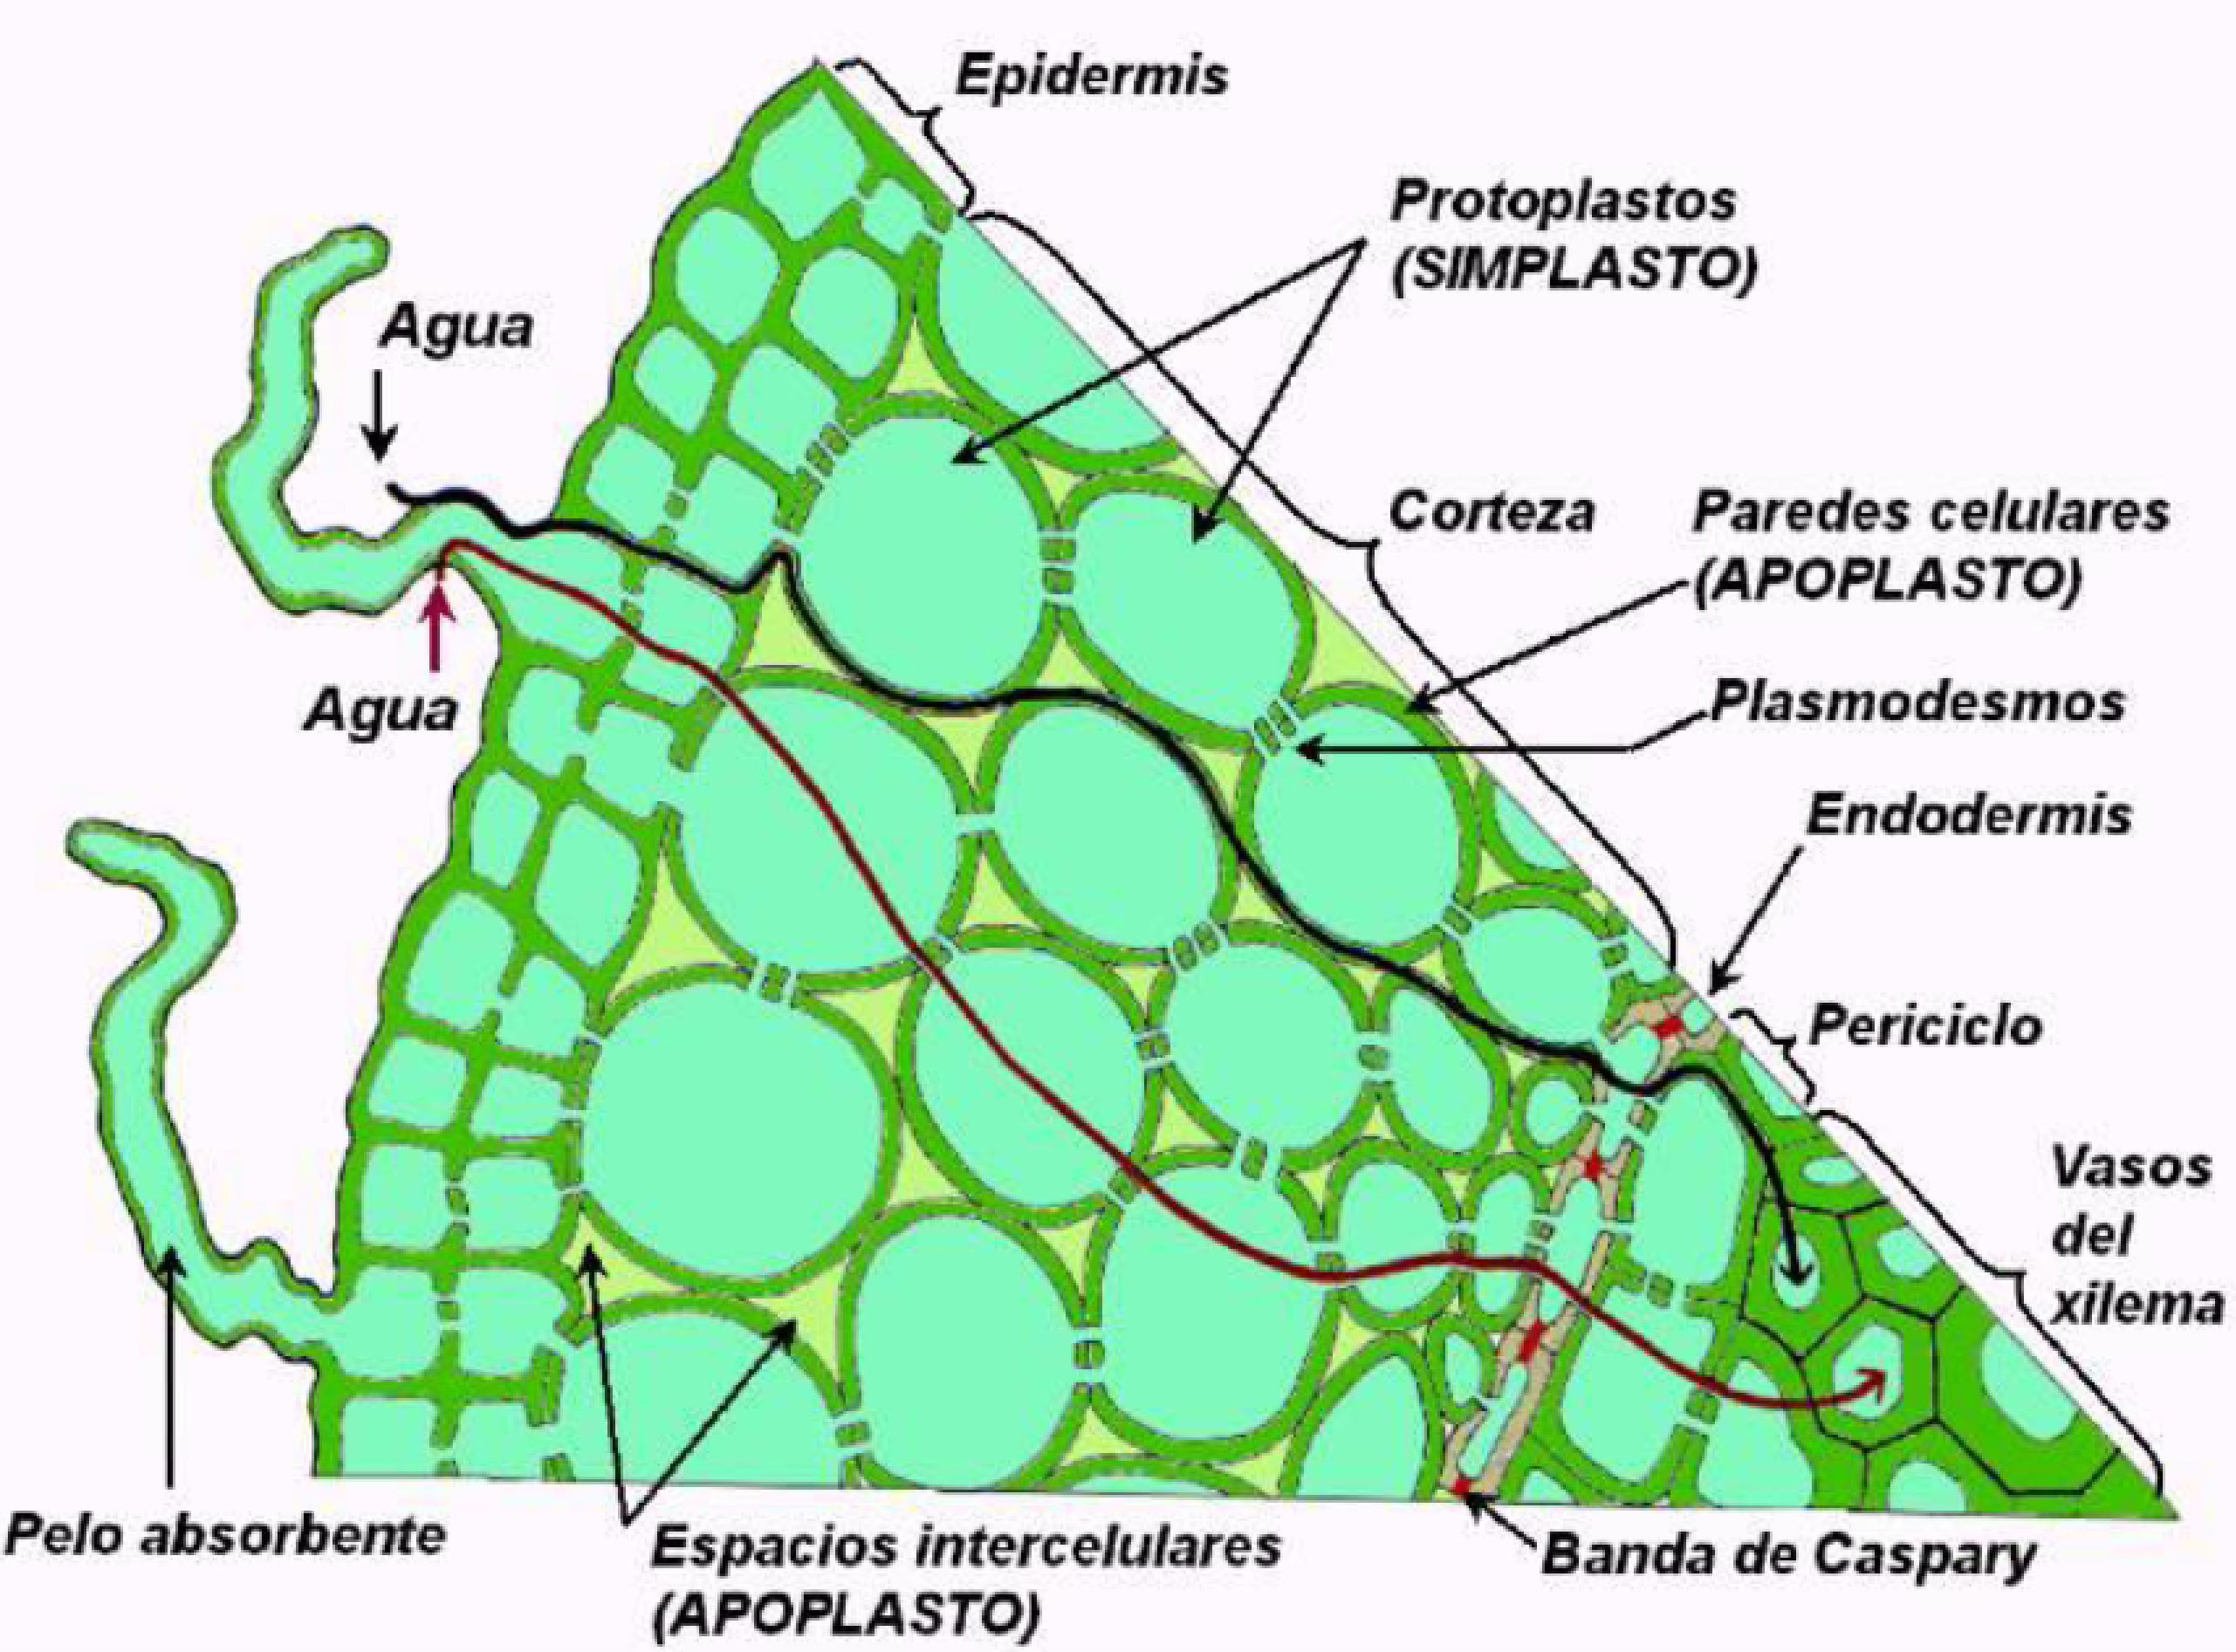
\includegraphics[width=0.5\textwidth]{fv1.png}}
  \caption{Intercambio entre célula y célula (Simplasto)}
  \label{fav1}
\end{figure}

\subsubsection{La banda de Caspary}
En la endodermis, el apoplasto está bloqueado por la banda de Caspary (formada por suberina y lignina). Toda el agua que penetra por la raíz se ve forzada a entrar en la vía simplástica a nivel de la endodermis.
Al llegar a la endodermis, el agua y los materiales que vienen por vía apoplástica, no pueden seguir debido a la presencia de la banda de Caspary. Son obligados a presentar en el protoplasto de las células endodérmicas y seguir la vía simplástica
hasta atravesar esta capa. El agua y los materiales que vienen por vía simplasto no ven alterado su camino.
\subsubsection{pH}
El agua pura tiene la capacidad de disociarse en iones, por lo que se puede considerar una mezcla de agua molecular, protones hidratados e iones hidroxilo.
Esta disociación es débil (para el agua pura), así el producto iónico del agua a $25^{\circ}C$ es: 
\begin{equation}
    K_w=[H^+][OH^-]=1.0\times 10^{-14}
\end{equation}

\begin{figure}[h!]
    \centerline{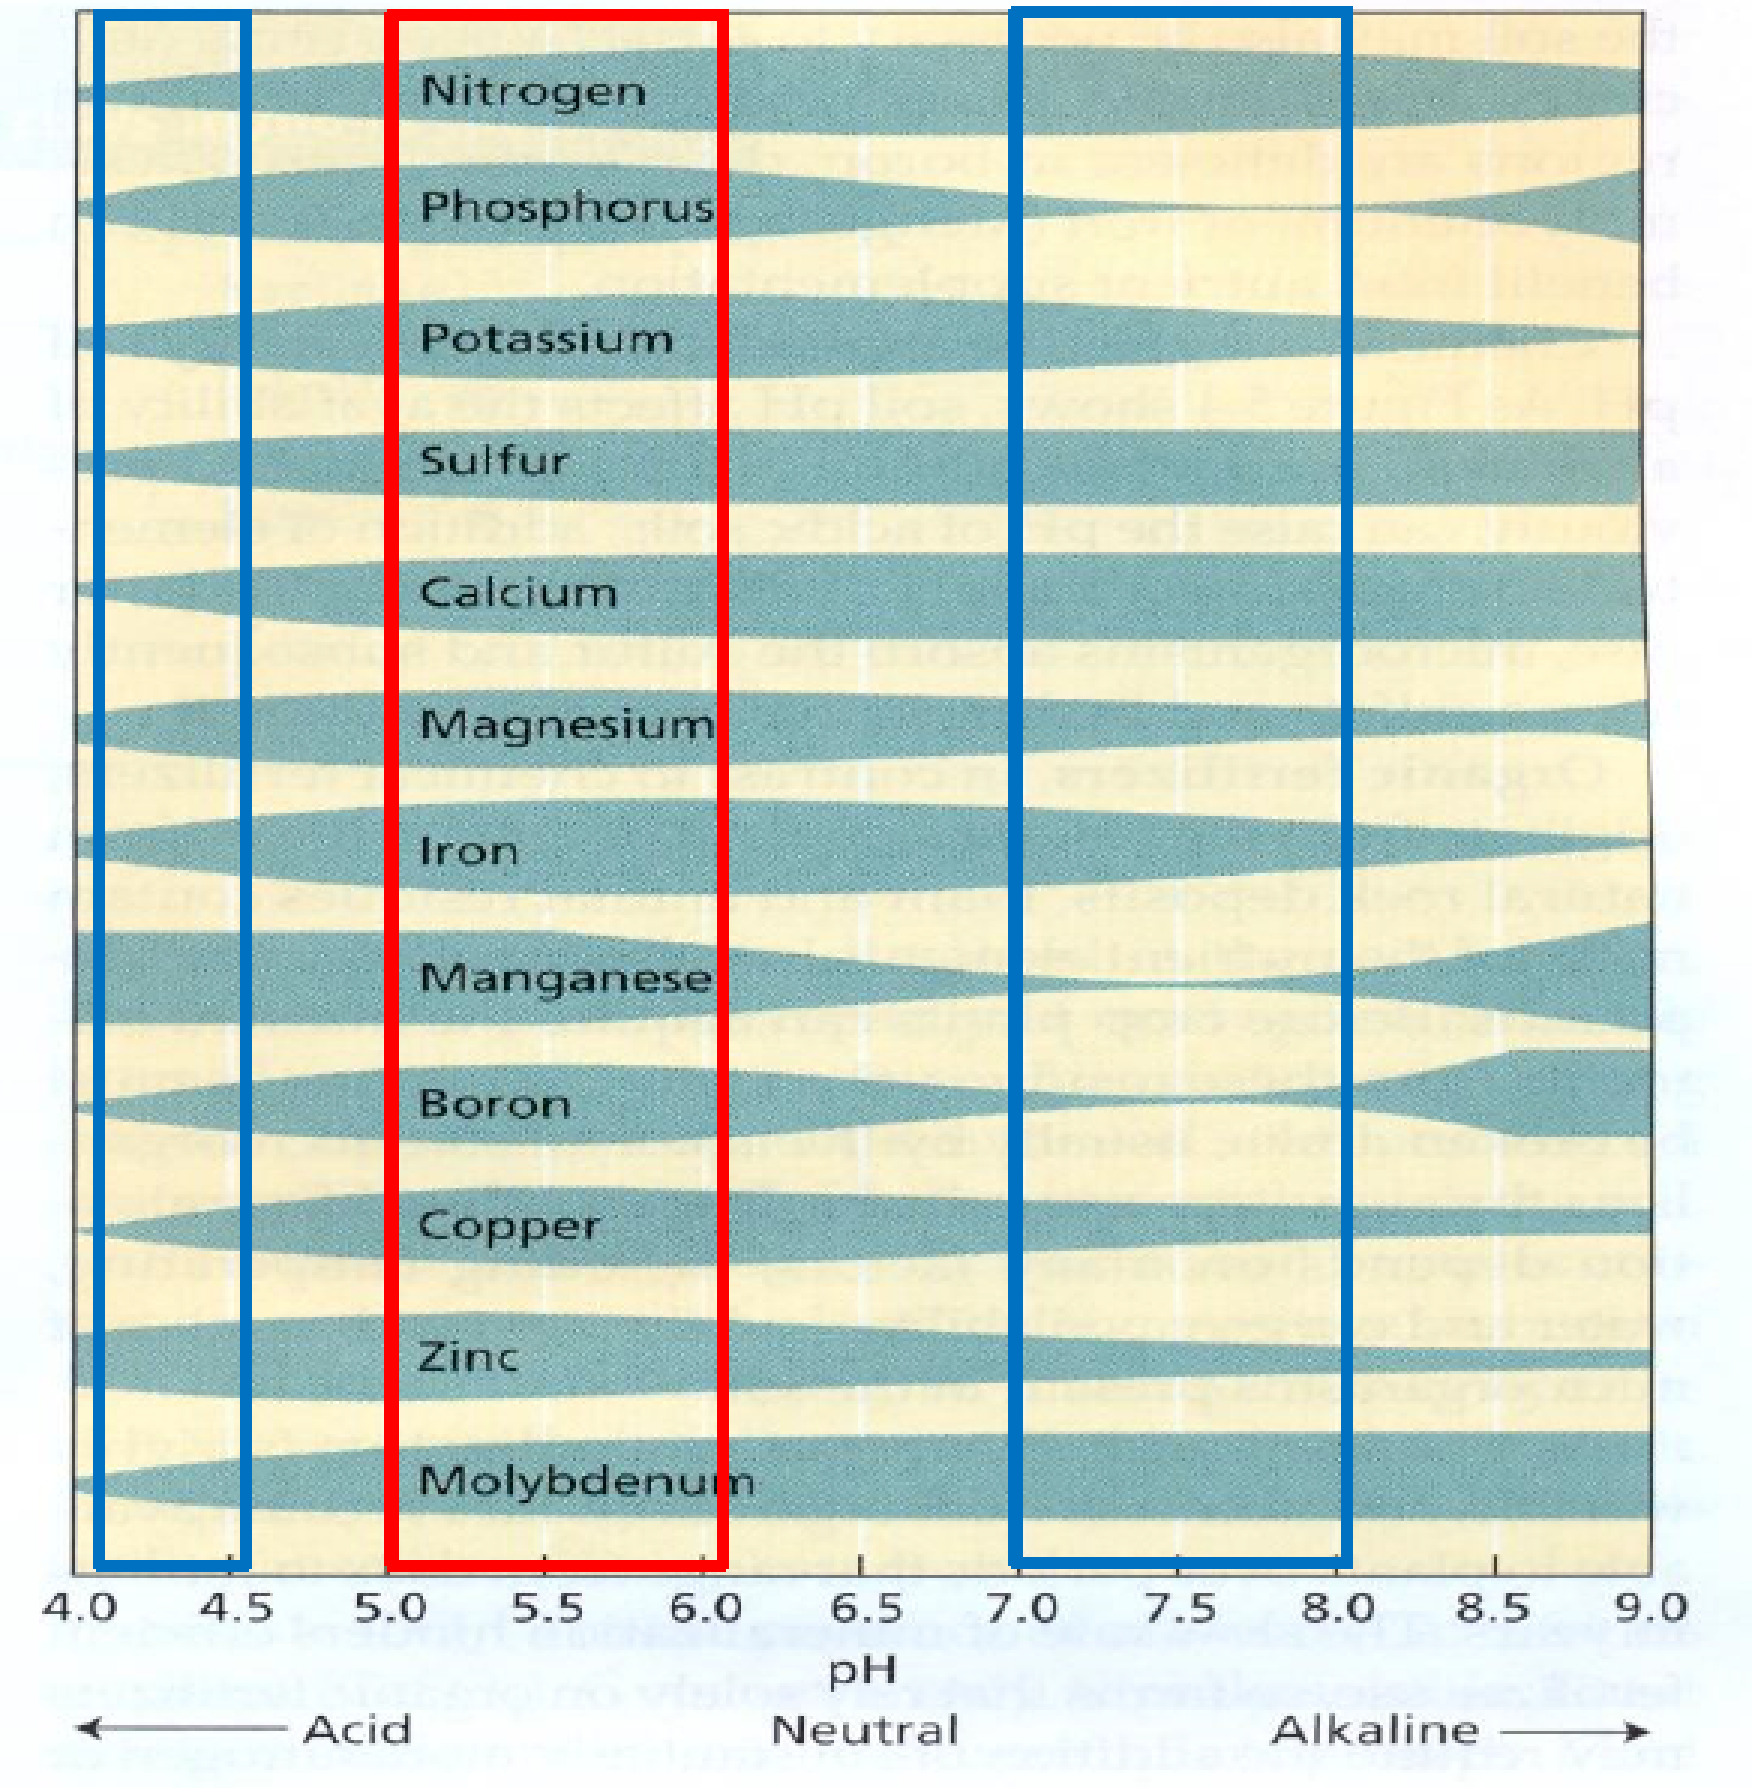
\includegraphics[width=0.5\textwidth]{fv2.png}}
    \caption{Relación del pH y la nutrición de macro y microelementos}
    \label{fav2}
  \end{figure}

Se puede tener nutrientes en el suelo, pero al tener un pH muy alcalino o ácido, la planta no podrá obtener éstos nutrientes. Por lo que se debe manejar el pH adecuado por especie.

\begin{figure}[h!]
    \centerline{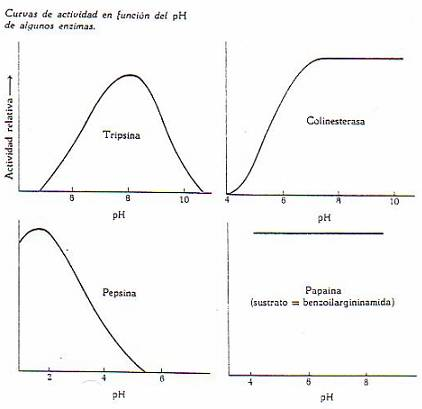
\includegraphics[width=0.5\textwidth]{fv3.jpg}}
    \caption{Curvas de actividad enzimática en función del pH}
    \label{fav3}
  \end{figure}

Las enzimas regulan diferentes reacciones metabólicas (véase la figura \ref{fav3}). El proceso de respiración vegetal, se lleva a cabo por cerca de 30 enzimas y es afectada por factores como temperatura y pH, el cual será abordado más adelante.


En la fotosíntesis, una enzima llamada \texttt{RuBisCO} encontrada en los cloroplastos de la célula vegetal, fija el $CO_2$ para formar azúcares y funciona en un pH cercano a 8

\begin{definition}[Capa de solvatación]
    Es una capa de moléculas de agua que cumple la función de disolver los iones de sodio y cloro (Aunque la orientación es distinta en ambos iones)
\end{definition}

\begin{figure}[h!]
    \centerline{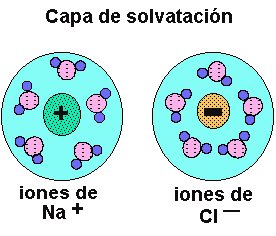
\includegraphics[width=0.5\textwidth]{fv4.png}}
    \caption{Diferencia por orientación por las leyes de cargas: atracción y repulsión}
    \label{fav4}
  \end{figure}

\subsubsection{Alteraciones del agua}

El agua no contaminada, tiene colores rojizos, pardos, amarillentos y verdosos.
debido a los compuestos húmicos, férricos o los pigmentos verdes de las algas que contienen.

En el caso del olor y sabor del agua, de forma natural pueden ser fenoles, hidrocarburos, por cloro, materias orgánicas en descomposición esencias liberadas por algas u hongos;
para tener un punto de partida, el sabor salado se puede comparar de la siguiente manera

\begin{itemize}
    \item $NaCl$: 250 ppm Sabor detectable 
    \item $CaCl_2$: 1000 ppm Sabor ausente
    \item $MgCl_2$: 100 ppm Sabor ausente
\end{itemize}
\subsubsection{Conductividad eléctrica}
La capacidad que tienen las sales inorgánicas en solución (electrolitos) para conducir la corriente eléctrica

El agua pura no conduce la corriente, pero el agua salina sí. Los iones cargados positiva y negativamente son los que conducen la corriente y la cantidad conducida dependerá del número de iones presentes y de su movilidad, se miden en Siemens por metro $S/m$
y micromhos por centímetro ($mmho/cm$), el agua potable tiene una conductividad de 50 a $100\mu S/cm$, mientras que el agua de mar hasta $53000\mu S/cm$

Dentro de las disoluciones moleculares iónicas son buenos conductores los ácidos, bases y sales inorgánicas, pero la sacarosa, bencenos, hidrocarburos y carbohidratos son pésimos conductores orgánicos. La conductividad eléctrica es lo mismo que dureza, por lo que hay problemas de salinidad, nutrición y precipitación en los equipos industriales.

La sensibilidad de los cultivos a la salinidad es muy notable, la cebolla, la fresa, naranja y zanahoria son muy sensibles, la alfalfa, apio, arroz, brócoli, coliflor son moderadamente sensibles, la Soja, sorgo y trigo son moderadamente tolerantes y el algodón, cebada, espárrago y remolacha son tolerantes.

\begin{definition}[Dureza]Es la concentración de compuestos minerales que hay en una determinada cantidad de agua, en particular sales de magnesio y calcio. 
    Se clasifica en \textbf{dureza temporal}
    producida  por carbonatos y puede ser eliminada al hervir el agua o por la adición de $CaOH$ (hidróxido de calcio).
\begin{equation}
    CaCO_{3(s)}+H_2O_{(l)}+CO_{2(g)}\rightleftharpoons Ca(HCO_3)_{2(aq)}
\end{equation}
Mientras que también está la \textbf{dureza permanente} no puede ser eliminada al hervir el agua y es causada por sulfato de calcio, magnesio y cloruros. Puede ser eliminada utilizando el método SODA (Sulfato de sodio)
\end{definition}

El carbonato de calcio es menos soluble en agua caliente que en agua fría, así que hervir
( contribuye a la formación de carbonato) se precipitará el bicarbonato de calcio fuera de la
solución, dejando el agua menos dura.

Los carbonatos pueden precipitar cuando la concentración de
ácido carbónico disminuye, con lo
que la dureza temporal disminuye, y si el ácido carbónico aumenta puede aumentar la solubilidad
de fuentes de carbonatos, como piedras calizas, con lo que la dureza temporal aumenta.
Todo esto está en relación con el pH de equilibrio de la calcita y con la alcalinidad de los
carbonatos. Este proceso de disolución y precipitación es el que provoca las formaciones de
estalagmitas y estalactitas

Las medidas de dureza o grado hidrotimétrico del agua son:

$mg\, CaCO_3 /L$ o ppm de $CaCO_3$

\begin{itemize}
    \item Grado alemán (Deutsche Härte , $dH^{\circ}$) Equivale a 17.9 mg $CaCO_3$ /L de agua.
    \item Grado americano Equivale a 17,2 mg $CaCO_3$ /L de agua.
    \item Grado francés ($f^{\circ}$) Equivale a 10,0 mg $CaCO_3$ /L de agua.
    \item Grado inglés ($e^{\circ}$) Equivale a 14.3 mg $CaCO_3$ /L de agua. 
\end{itemize}

Un proceso para la eliminación de la dureza del agua, es la descalcificación de ésta mediante resinas intercambiadoras de iones

Lo más habitual es utilizar resinas aniónicas que intercambian iones sodio por los iones calcio y magnesio presentes en el agua.

La dureza también se puede percibir por el sabor del agua.

Es conveniente saber si el agua es agua dura, porque puede provocar depósitos de carbonatos en conducciones de lavadoras , calentadores, y calderas o en las planchas Para diluir los carbonatos, aplicar un ácido débil (acético, cítrico) en los depósitos.

Las alteraciones biológicas del agua, pueden producir enfermedades mortales tanto para el humano, como para las plantas y están dadas por: 
\begin{itemize}
    \item Bacterias
    \item coliformes
    \item Desechos fecales
    \item Virus
    \item Desechos fecales y restos orgánicos
    \item Animales, plantas, microorganismos diversos
    \item Eutrofización
\end{itemize}


\subsubsection{Transporte}

\begin{definition}[Transporte Pasivo]
    Se da en función de diferencias en concentración, temperatura y altura
(sin gasto de energía). Osmosis, difusión y flujo masivo
\end{definition}

\begin{definition}[Transporte Activo]
    Se da considerando un gasto de energía
\end{definition}


El transporte de agua se da gracias a las \textbf{acuaporinas}, la cual es una proteína que
junto al sistema vascular de la planta o animales, permite la regulación del fluido hídrico. 

\subsubsection{Potencial hídrico}

\begin{definition}[Potencial hídrico]
    Define a la capacidad que tiene el agua de moverse de un lugar a otro; es preciso entender el sistema suelo agua planta atmósfera:
    permite predecir cómo se moverá el agua bajo diversas condiciones. El agua se mueve de forma espontánea desde una zona de potencial hídrico grande a una zona con el potencial menor, independientemente de la causa que provoque esta diferencia, se mueve de mayor potencial a menor potencial
\end{definition}

El potencial hídrico ($\psi $) se puede expresar en función de sus componentes:
\begin{equation}
\psi=\psi_p+\psi_o+\psi_m+\psi_g
\end{equation}

\begin{itemize}
    \item $\psi$ Potencial hídrico
    \item $\psi_p$ Potencial de presión o turgencia
    \item $\psi_o$ Potencial osmótico o de solutos
    \item $\psi_m$ Potencial matricial
    \item $\psi_g$Potencial de gravedad
\end{itemize}

El agua pura tiene un potencial hídrico de cero atmósferas (atm) a $21^{\circ}C$, si la temperatura aumenta, también aumenta su potencial y viceversa con signo negativo.
A medida que la planta presenta estrés o está sin agua, la síntesis de ácido abscísico y la concentración o acumulación de solutos aumenta, mientras que la fotosíntesis, síntesis de proteínas, paredes celulares, expansión celular y conductancia de los estomas disminuyen a comparación de cuando tiene un potencial en 0.

\subsubsection{El potencial Presión}
El potencial de presión es nulo a presión atmosférica, es positivo sobre presiones por encima de la atmosférica y negativo en condiciones de tensión o vacío, esto afecta principalmente a la turgencia de las hojas.

\subsubsection{El potencial Osmótico}

Representa la disminución de la capacidad de desplazamiento del agua debido a la presencia de solutos.

A medida que la concentración de solutos (es decir, el número de partículas de soluto por unidad de volumen de la disolución) aumenta, el potencial osmótico se hace negativo

Sin la presencia de otros factores que alteran el potencial hídrico, las moléculas de agua de las disoluciones se moverán desde lugares con poca concentración de soluto.

\subsubsection{El potencial matricial}

Representa el grado de retención del agua, debido a las interacciones con matrices sólidas o coloidales, puede valer cero, si no hay interacciones, o ser negativo.

\subsubsection{Formas de agua en el suelo}

\begin{definition}[Agua de combinación química]
    Forma parte de compuestos químicos, como la limonita $Fe_2O_3\times 2H_2O$. Esta agua no es disponible para las plantas y biológicamente inactiva
\end{definition}

\begin{definition}[Agua hidroscópica]
    Es agua contenida en los suelos secos al aire, aquella que está en equilibrio con la humedad ambiente. Inactiva biológicamente
\end{definition}

\begin{definition}[Agua capilar]
    Agua contenida en los microporos del suelo. Disponible para las plantas y biológicamente activa
\end{definition}

\begin{definition}[Agua gravitacional (no capilar)]
    Agua contenida en los macroporos del suelo y que drena por la fuerza de gravedad (agua de drenaje). Si su movimiento es lento, puede ser utilizada por las plantas
\end{definition}

\subsubsection{Capacidad de retención de agua por el suelo}

\begin{definition}[Saturación]
    Suelo totalmente lleno de agua, las plantas se ahogan por falta de aire
\end{definition}

\begin{definition}[Capacidad de campo]
    Cuando el suelo evacua el agua por gravedad, pero continúa húmedo.
\end{definition}

\begin{definition}[Punto de marchitez permanente]
    Agua del suelo a la cual la planta no puede acceder,por lo tanto se marchita y muere.
\end{definition}


\begin{table}[h!]
    \centering
    \begin{tabular}{@{}cc@{}}
    \toprule
    Textura del suelo & Velocidad de infiltración (mm/h) \\ \midrule
    Suelo Arcilloso   & 1-5                              \\
    Suelo limoso      & 8-12                             \\
    Suelo arenoso     & 25-50                            \\ \bottomrule
    \end{tabular}
    \caption{Velocidad de infiltración del agua según la textura del suelo. UNAM. Ingeniería de Riego y Drenaje 1979}
    \label{tabfv1}
    \end{table}

    \begin{table}[h!]
        \centering
        \begin{tabular}{@{}ccccc@{}}
        \toprule
        \multirow{2}{*}{Textura}& \multicolumn{4}{c}{Tensión (atm)} \\
                                & 0.3    & 1.0    & 5.0    & 15.0   \\ \midrule
        Arcilla                 & 34.2   & 27.2   & 21.8   & 17.5   \\
        Arcillo-arenoso         & 29.8   & 20.3   & 18.4   & 16.5   \\
        Franco arenoso          & 10.8   & 73     & 6.2    & 5.4    \\ \bottomrule
        \end{tabular}
        \caption{Porcentaje de humedad a diferentes tensiones en tres tipos de suelo}
        \label{tabfv2}
        \end{table}

\subsubsection{Ajuste osmótico}

No tiene carga neta a pH fisiológico, tampoco tóxicos a altas concentraciones y se acumulan en el citoplasma, altamente solubles.

\subsection{Nutrientes esenciales}

Criterios de esencialidad
\begin{enumerate}
    \item La deficiencia del elemento M, impide que la planta complete su ciclo vital
    \item El elemento M debe participar directamente en el metabolismo de la planta
    \item El elemento M no debe ser reemplazado por otro que tiene propiedades similares
\end{enumerate}

Puede decirse que el Carbono, hidrógeno y oxígeno ocupan cerca del 96\% de la nutrición vegetal, además que ya están dados.
Los macronutrientes ocupan el 0.5\%, enlistados por:
\begin{itemize}
    \item Hierro
    \item Cloro
    \item Manganeso
    \item Boro
    \item Zinc
    \item Cobre
    \item Molibdeno
\end{itemize}
Mientras que los macronutrientes:
\begin{itemize}
    \item Nitrógeno
    \item Potasio
    \item Fósforo
    \item Magnesio
    \item Azufre
\end{itemize}


\begin{table}[h!]
    \centering\begin{tabular}{@{}lllll@{}}
    \toprule
    Elemento  & \begin{tabular}[c]{@{}l@{}}Símbolo\\ Químico\end{tabular} & \begin{tabular}[c]{@{}l@{}}Forma\\ disponible\end{tabular} & \begin{tabular}[c]{@{}l@{}}Conc.\\ (mg/kg)\end{tabular} & Funciones                                                                                                                                                                                                                                                       \\ \midrule
    Nitrógeno & N                                                         & $NO_3^-$, $NH_4^+$                                         & 15000                                                   & \begin{tabular}[c]{@{}l@{}}El nitrógenos es el componente de los aminoácidos, de los ácidos\\ nucléicos, de los nucleótidos, de la clorofila y de las coenzimas\end{tabular}                                                                                    \\
    Potasio   & K                                                         & $K^+$                                                      & 10000                                                   & \begin{tabular}[c]{@{}l@{}}El potasio se intercambia por ósmosis y el equilibrio iónico, así\\ como en la apertura y el cierre de los estomas; activa también de\\ numerosas enzimas\end{tabular}                                                              \\
    Calcio    & Ca                                                        & $Ca^+$                                                     & 5000                                                    & \begin{tabular}[c]{@{}l@{}}Es un componente de la pared celular; cofactor de enzimas;\\ interviene en la permeabilidad de las membranas celulares;\\ componiendo la calmodulina, regulador de actividades enzimáticas y\\ también de las membranas\end{tabular} \\
    Magnesio  & Mg                                                        & $MG^{2+}$                                                  & 2000                                                    & \begin{tabular}[c]{@{}l@{}}Es un componente de clorofila; activador de numerosas\\ enzimas\end{tabular}                                                                                                                                                         \\
    Fósforo   & P                                                         & $H_2PO^-_4$                                                & 2000                                                    & \begin{tabular}[c]{@{}l@{}}Se encuentra el fósforo en los compuestos fosfatados que transportan\\ energía (ATP,ADP), los ácidos nucléicos varias coenzimas y los\\ fosfolípidos\end{tabular}                                                                    \\
    Azúfre    & S                                                         & $SO_4^{2-}$                                                & 1000                                                    & \begin{tabular}[c]{@{}l@{}}El azufre forma parte de algunos aminoácidos (cisteína, metionina),\\ así como de la coenzima A\end{tabular}                                                                                                                         \\ \bottomrule
    \end{tabular}
    \caption{Macronutrientes }
    \label{tabfv3}
\end{table}

\begin{table}[h!]
    \centering
    \begin{tabular}{@{}lllll@{}}
        \toprule
        Elemento  & \begin{tabular}[c]{@{}l@{}}Símbolo\\ Químico\end{tabular} & \begin{tabular}[c]{@{}l@{}}Forma\\ disponible\end{tabular} & \begin{tabular}[c]{@{}l@{}}Conc.\\ (mg/kg)\end{tabular} & Funciones                                                                                                                                                                                 \\ \midrule
        Cloro     & Cl                                                        & $Cl^-$                                                     & 100                                                     & \begin{tabular}[c]{@{}l@{}}El cloro se produce en la ósmosis y el equilibrio iónico; es\\ indispensable para las reacciones fotosintéticas que producen\\  el oxígeno\end{tabular}        \\
        Hierro    & Fe                                                        & $Fe^{3+}$, $Fe^{2+}$                                       & 100                                                     & \begin{tabular}[c]{@{}l@{}}El hierro es necesario para la síntesis de la clorofila;\\ componente de los citocromos y de las nitrogenasa\end{tabular}                                      \\
        Boro      & B                                                         & $H_4BO_3$                                                  & 20                                                      & \begin{tabular}[c]{@{}l@{}}El boro interviene en la utilización del calcio, la síntesis de\\ los ácidos nucléicos y la integridad de las membranas\end{tabular}                           \\
        Manganeso & Mn                                                        & $Mn^{2+}$                                                  & 50                                                      & \begin{tabular}[c]{@{}l@{}}Es activador de algunas enzimas; necesario\\ para la integridad de la membrana cloroplástica y para la\\ liberación de oxígeno en la fotosíntesis\end{tabular} \\
        Zinc      & Zn                                                        & $Zn^{2+}$                                                  & 20                                                      & Es el activador o componente de numerosas enzimas                                                                                                                                         \\
        Cobre     & Cu                                                        & $Cu^+$, $Cu^{2+}$                                          & 6                                                       & \begin{tabular}[c]{@{}l@{}}Es el activador o componente de algunas enzimas\\ que se producen en las oxidaciones y las reducciones\end{tabular}                                            \\
        Níquel    & Ni                                                        & $Ni^{2+}$,  $MoO_4^{2-}$                                   & -                                                       & \begin{tabular}[c]{@{}l@{}}Forma la parte esencial de una enzima que\\ funciona en el metabolismo\end{tabular}                                                                            \\
        Molibdeno & Mo                                                        &                                                            & 0.1                                                     & \begin{tabular}[c]{@{}l@{}}Es necesario para la fijación del nitrógeno y en la reducción \\ de los  nitratos\end{tabular}                                                                 \\ \bottomrule
        \end{tabular}
        \caption{Micronutrientes}
        \label{tabfav4}
\end{table}

\begin{table}[h!]
    \centering
    \begin{tabular}{@{}ll@{}}
    \toprule
    Micronutrientes & Función                                                                                                                                                     \\ \midrule
    Fe,Mn,Cu,Ni     & \begin{tabular}[c]{@{}l@{}}Constituyente de enzimas\\ (metalproteínas)\end{tabular}                                                                         \\
    Mn,Zn           & Activación de enzimas                                                                                                                                       \\
    Fe,Cu,Mn(Cl)    & \begin{tabular}[c]{@{}l@{}}Involucrado en el transporte\\ de electrones en la fotosíntesis\end{tabular}                                                     \\
    Mn,Zn,Mo        & \begin{tabular}[c]{@{}l@{}}Involucrado en la tolerancia al\\ estrés\end{tabular}                                                                            \\
    Cu, Mn,Zn,B     & \begin{tabular}[c]{@{}l@{}}Involucrado en el crecimiento\\ reproductivo (inducción a la\\ floración, polinización,\\ establecimiento de fruto)\end{tabular} \\
    B.Zn            & \begin{tabular}[c]{@{}l@{}}Constituyente de paredes \\ celulares y membrana\end{tabular}                                                                    \\ \bottomrule
    \end{tabular}
    \caption{Principales funciones de los micronutrientes de las plantas}
    \label{tabfv5}
\end{table}

\section{Fotosíntesis}
\textbf{Fotosíntesis Oxigénica}
\begin{equation}
    H_2O\longrightarrow 2H^++2e^-+\frac{1}{2}O_2
\end{equation}
Es producida por plantas superiores, como algas y cianobacterias

\textbf{Fotosíntesis anoxigénica}
\begin{equation}
    H_2S\longrightarrow 2H^++e^-+S
\end{equation}
Aquí lo producen bacterias, purpúreas y verdes del azufre,
sin embargo la ecuación más popular que describe a la fotosíntesis es la siguiente: 

\begin{equation}
    6CO_2+6H_2O\longrightarrow C_6H_{12}O_6+6O_2
\end{equation}

\smartdiagram[circular diagram]{
	Mediante el $CO_2$ y $H_2O$, Se produce la fotosíntesis, Se forma glucosa y $O_2$, Respiración y energía}

Se dice que durante el día y la noche ocurren procesos diferentes. Lo cierto es que durante el día, hay un intercambio entre el oxígeno y el dióxido de carbono y al mismo tiempo se absorbe el agua. DUrante la noche hay una absorción de microelementos y macroelementos

\begin{definition}[Luz blanca]
    La luz blanca es una mezcla de colores diferentes que van desde el violeta hasta rojo por la diversidad de las longitudes de onda
\end{definition}

La fotosíntesis se divide entre la fase luminosa y la fase enzimática. En el interior del cloroplasto, se encuentran tilacoides apilados unos con otros (Grana) y están cubiertas con un material llamado Lumen.
Los complejos antena o complejos colectores de luz presentes en los cloroplastos funcionan como un embudo; colectan los fotones y transfieren la energía hasta los centros de reacción, en la figura \ref{fv5}, puede
ser entendida en tres partes: La fotólisis del agua es el rompimiento de la molécula del agua, pasa por un complejo enzimático para generar $O_2$, $H^+$ junto con electrones libres para hacer una transferencia de $e^-$, la segunda parte la Plastoquinona adquiere los electrones, para luego cederlos al citocromo, luego a la plastocianina (que recibe más energía), se transportan a la ferredoxina para finalmente dárselos a la ferredoxina NADP + reductasa, donde se produce el NADH.H, es el último receptor de los electrones.
Al final, todos los $H^-$ se almacenan en el tilacoide; El tercer paso es la síntesis del ATP.

\begin{figure}[h!]
\centering
  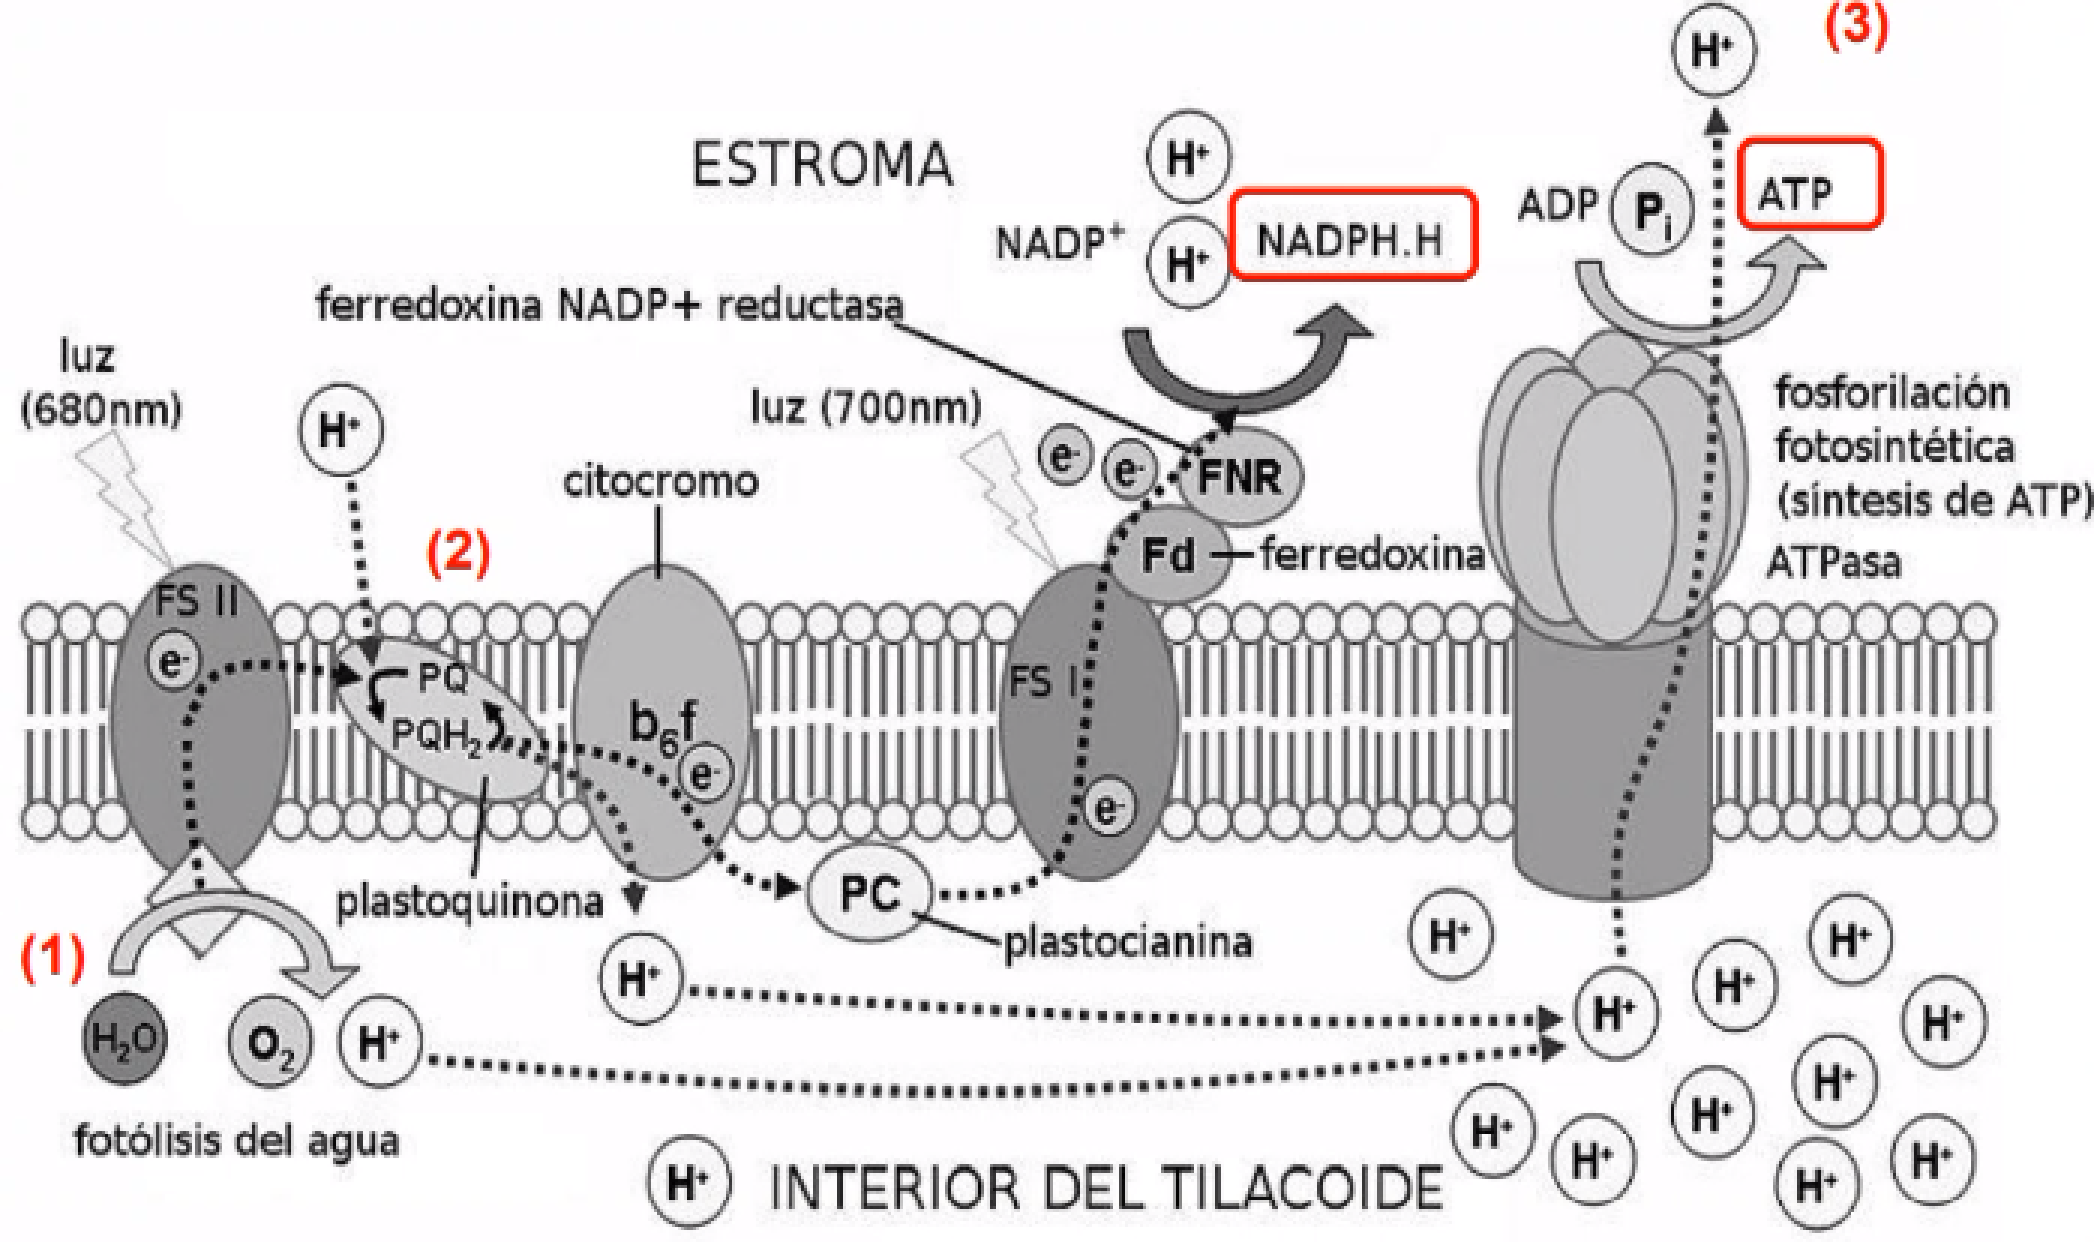
\includegraphics[width=0.5\textwidth]{fv5.png}
  \caption{Esquema de la etapa luminosa, que se produce en los tilacoides}
  \label{fv5}
\end{figure}

\subsection{Ciclo de calvin}

Es una serie de reacciones para saber cómo se fija el $CO_2$ para producir glucosa.

\begin{figure}[h!]
    \centering
      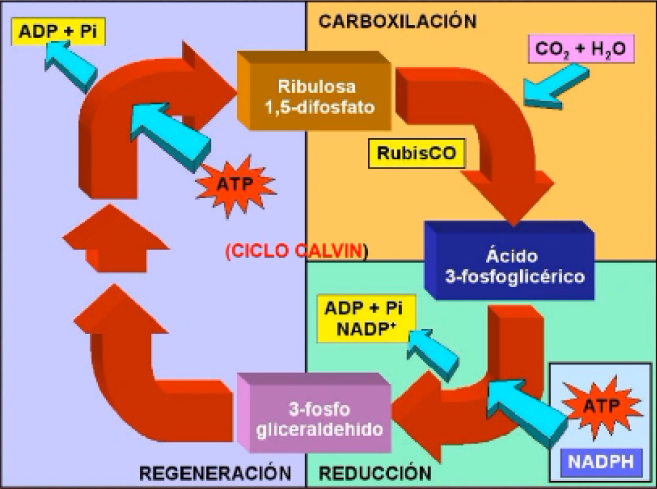
\includegraphics[width=0.5\textwidth]{fv6.png}
      \caption{Esquema del ciclo de Calvin con las tres etapas}
      \label{fv6}
    \end{figure}


Carboxilación: Tiene que ver con la fijación del carbono por una enzima que se llama RubisCO, llamado así por la ribulosa carboxilasa/oxigenasa.
por medio del $CO_2$ y $H_2O$ y el RubisCO, produce el ácido 3-fosfoglicérico.
Por medio del ATP se transforma en 3-fosfogliceraldehido con ADP6Pi $NADP^+$ que a su vez crea la ribulosa 1,5 difosfato 

\begin{figure}[h!]
    \centering
      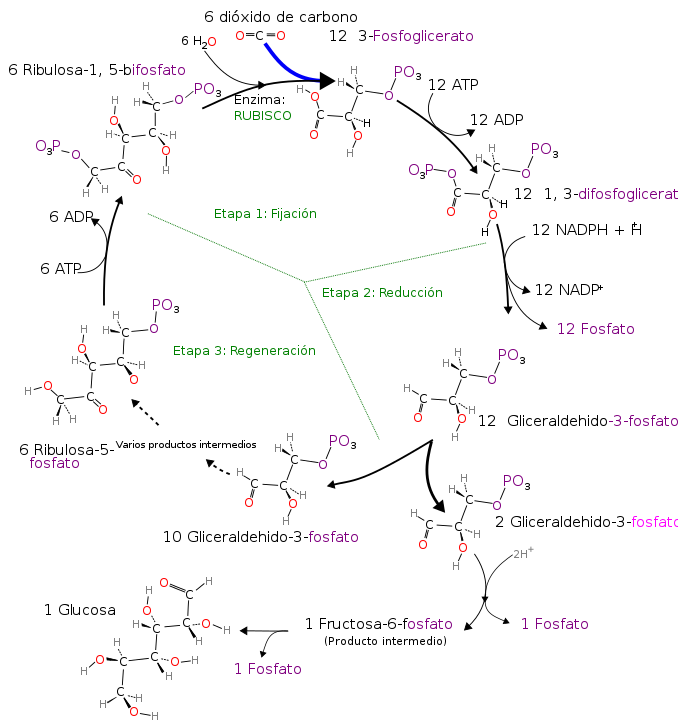
\includegraphics[width=0.5\textwidth]{fv7.png}
      \caption{Esquema del ciclo de Calvin completo}
      \label{fv7}
    \end{figure}

La primer modificación que hacen las plantas son a nivel anatómico,

\begin{figure}[h!]
    \centering
      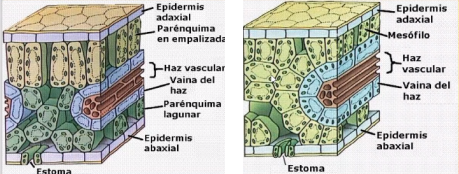
\includegraphics[width=0.5\textwidth]{fv8.png}
      \caption{En la izquierda, características anatómicas de una planta C3 y en la derecha una planta C4}
      \label{fv8}
\end{figure}

\begin{figure}[h!]
    \centering
      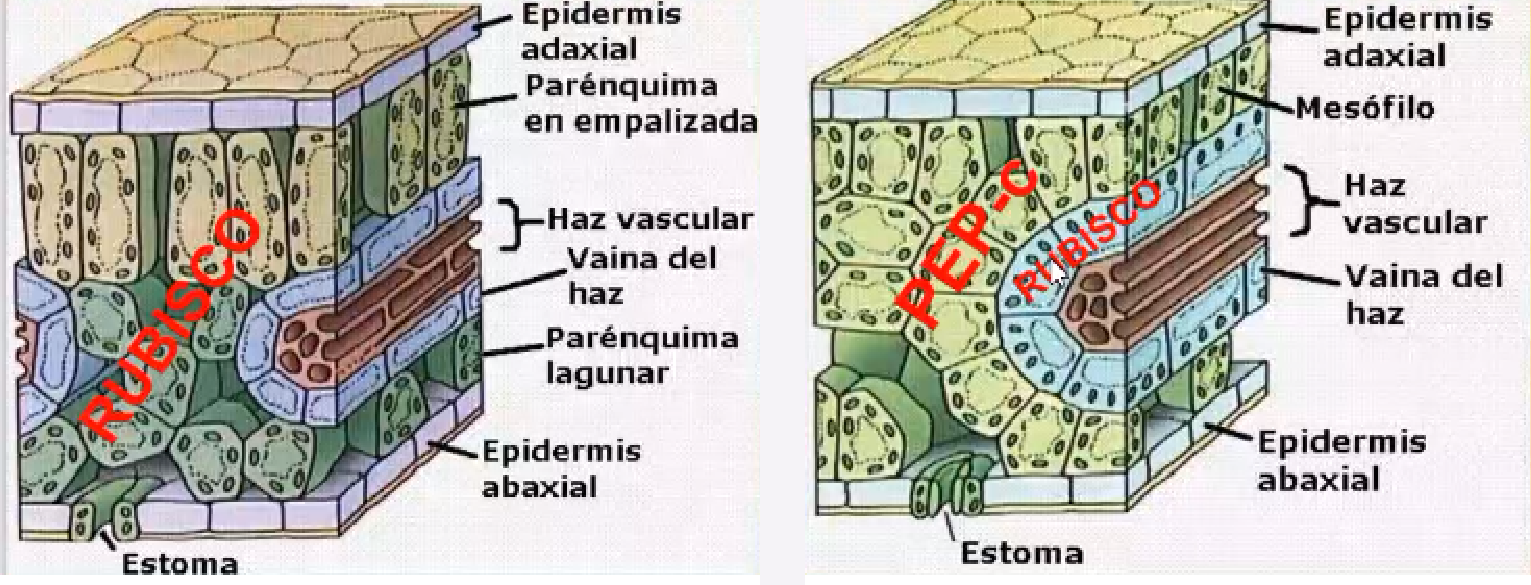
\includegraphics[width=0.5\textwidth]{fv9.pdf}
      \caption{Esquema de la anatomía típica de una planta C3 (izquierda) y C4 (derecha)}
      \label{fv9}
\end{figure}
\subsection{Metabolismo y respiración}

\begin{definition}[Anabolismo]
    Síntesis de compuestos
\end{definition}
\begin{definition}[Catabolismo]
    Degradación de compuestos
\end{definition}
Existen dos tipos de metabolismos, el anabolismo y el catabolismo.

La importancia del proceso respiratorio implica: 
\begin{enumerate}
    \item Aporta energía necesaria para el metabolismo celular
    \item Contribuye a la síntesis de intermediarios y compuestos químicos
    \item Liberación de energía
    \item Favorece la interconversión de compuestos como: \begin{align*}
        &\text{Almidón}\longrightarrow \text{Azúcares}\\
        &\text{Azúcares}\longrightarrow \text{Ácidos orgánicos}\\
        &\text{Ácidos grasos} \longrightarrow \text{Proteínas}\\
        &\text{Ácidos orgánicos}\longrightarrow \text{Proteínas}\\
        &\text{Ácidos orgánicos}\longrightarrow \text{Ácidos orgánicos}
    \end{align*}
    \item Síntesis de compuestos tóxicos (Etanol y Acetaldehídos)
    \item Síntesis de compuestos volátiles ($CO_2$ y aromas)
\end{enumerate}

\begin{equation}
    C_6H_{12}O_6+6O_2\longrightarrow 6H_2O+6CO_2+686\,KCal
\end{equation}
La ecuación de la respiración, consiste en tres etapas:
\begin{enumerate}
    \item Glicólisis (Citoplasma)
    \item Ciclo de Krebs (Matriz de la mitocondria)
    \item Transporte de electrones (Crestas de la membrana interna de la mitocondria)
\end{enumerate}

La respiración anaeróbica es un proceso biológico de oxidorreducción de monosacáridos y otros compuestos en el que el aceptor terminal de electrones es una molécula inorgánica distinta del oxígeno y más raramente una molécula orgánica.

La realizan exclusivamente algunos grupos de bacterias y para ello utilizan una cadena transportadora de electrones análoga a la de la mitocondria en la respiración aeróbica. No debe confundirse con la fermentación, que es un proceso también anaeróbico, pero en el que no participa nada parecido a una cadena transportadora de electrones y el aceptor final de electrones es siempre una molécula orgánica.

\begin{definition}[Cociente respiratorio]
    Es la relación entre el $CO_2$ desprendido y el $O_2$ absorbido durante la respiración
    \begin{equation}
        C_r = \frac{CO_2}{O_2}
    \end{equation}
\end{definition}

Para la glucosa o fructosa, $C_r=1$
\begin{equation}
    C_6H_{12}O_6 + 6O_2 \longrightarrow 6CO_2 + 6H_2O
\end{equation}
Ácidos orgánicos, $C_r=1$
\begin{equation}
    2\left( C_6H_8O_7 \right) + 9O_2 \longrightarrow 12CO_2 + 8H_2O
\end{equation}

Y los ácidos grasos o aminoácidos, $C_r\leq 1$ pues $\frac{18CO_2}{26O_2}=0.7$
\begin{equation}
    C_{18}H_{36}26O_2 \longrightarrow 18CO_2 + 18H_2O
\end{equation}

\subsection{Hormonas}

\subsection{Metabolitos secundarios}

Son compuestos químicos sintetizados por las plantas que cumplen funciones no esenciales en ellas, de forma que su ausencia no es letal para ellas

La importancia es por la producción  de drogas medicinales, venenos, saborizantes, pegamentos, aceites, ceras, antibióticos, insecticidas y herbicidas entre otros materiales

\begin{enumerate}
    \item Terpenoides. Se conocen más de 25 000 compuestos.
    \item Compuestos fenólicos y sus derivados, Los más de 8000 compuestos fenólicos conocidos se sintetizan por la ruta del ácido shikímico o por la del malonato/acetato.
    \item Compuestos nitrogenados o alcaloides. Se conocen alrededor de 12,000 alcaloides. Ejemplos conocidos son la cocaína, la morfina, la atropina, la colchicina, la quinina, y la
\end{enumerate}

Las hormonas derivadas de Aminoácidos son:
\begin{itemize}
    \item Triptofano genera auxinas
    \item Metionina genera Etileno
    \item Arginina genera poliaminas
\end{itemize}
Las hormonas derivadas de Terprenos:
\begin{itemize}
    \item Citocininas
    \item Giberelinas
    \item Brassinoesteroides
    \item Ácido abscísico
\end{itemize}

Ejemplos y Funciones Generales de Metabolitos Secundarios

Hormonas Tradicionales (GA, ABA, Cit. Terpenics);
Hormonas No- Tradicionales (Grastripesteroides Terpenos SA, C. Fenólion) Sintesis de Pigmentos Fotosintéticos (Kanturias Clomties JupENTS);
Constituyente Estructural (Lignite Atrayentes de Polinizadores en Angiospermas (Colores en flores: 20 Aromas Terpenos);
Defensa a microorganismos patógenos (Floaluxmasplapende, Of Famolice;
Defensa a insectos herbívoros (-celloides: Comp. Nitrogenados)
Interacciones alelopáticas.

Metabolitos primarios:
\begin{itemize}
    \item Azúcares
    \item Lípidos
    \item Nucleotidos
    \item Aminoácidos
    \item Fitoesteroles
    \item Intermediarios
\end{itemize}

\subsubsection{Monoterpenos}
Generan los aromas de las plantas, existen aceites esenciales como el limoleno y mentol.
\subsubsection{Diterpenos}
Entre los diterpenoides, se encuentran las giberelinas y el fitol, un diterpeno de cadena abierta que forma parte de la estructura de las clorofilas 
\subsubsection{Triterpenos}
El esterol más abundante de animales es el colesterol (Fig.10), presente también en plantas aunque en trazas, razón por la cual los aceites vegetales se etiquetan como ``libres de colesterol''.
La principal función de los esteroles en plantas es formar parte de las membranas y determinar su viscosidad y su estabilidad. Algunos esteroles tienen funciones protectoras frente a insectos como en el caso de la ecdisona aislada del helecho común

Los limonoides también son triterpenos, las sustancias amargas de los cítricos que actúan como anti herbívoros. Un limonoide de los más poderosos repelentes de insectos es la azadiractina que se usa en la industria alimentaria y en agronomía para el control de plagas.

La vitamina A es un grupo orgánicos nutricionales insaturados que incluyen metinol, retinal, ácido retinoico y caroteno).

varios carotenoides provitamina A (especialmente el beta)

La vitamina A tiene múltiples funciones: es importante para el crecimiento y el desarrollo, para el mantenimiento del sistema inmunológico y para una buena visión.

\subsubsection{Ácidos fenolicos}
Los ácidos fenólicos que tienen interés terapéutico son derivados del ácido benzoico o del ácido cinámico (cafeico, ferúlico, p-cumárico). Entre las plantas medicinales que poseen ácidos fenólicos vamos a destacar la alcachofa con actividad colerética, el ortosifón con actividad diurética y la equinácea empleada por sus propiedades inmunoestimulantes. Igualmente incluimos en este capítulo, plantas medicinales, reina de los prados y sauce, que poseen derivados del ácido salicílico con actividad antiinflamatoria, analgésica y antipirética.

\subsubsection{Cumarinas}
Como grupo, su interés farmacológico no es muy grande, sin embargo debemos mencionar sus efectos sobre el sistema vascular tanto en territorio arterial como venoso y su utilidad en el tratamiento de algunas alteraciones de la piel como por ejemplo la psoriasis debido a sus propiedades fotosensibilizantes. Ejemplo de este tipo de principios activos es la visnadina, piranocumarina con efectos vasodilatadores presente en el Amni visnaga. También antimicrobianos y anticoagulantes.\footnote{La propiedad física más importante de estos compuestos es la fluorescencia generada con la luz ultravioleta (365 nm), propiedad ampliamente usada para su detección.}

\subsubsection{Quinonas}
Las quinonas son muy abundantes en la naturaleza, en el Reino Vegetal se encuentran tanto en vegetales superiores como en hongos y bacterias. Las plantas que contienen estos compuestos son especies vegetales que pueden comportarse como laxantes o como purgantes según las dosis administradas. Las antraquinonas se encuentra en forma natural en algunas plantas (Espino Cerval y el género Aloe), hongos, líquenes Los derivados naturales de la antraquinona son glucósidos con acción laxante y purgante sumamente potente. En la terapéutica farmacológica, la antraquinona pertenece a la categoría de catárticos y se usan en la terapia contra el estreñimiento, Se encuentran en las hojas, vainas, raíces y semillas de diversas plantas como el sen, el ruibarbo y la frángula. Dependiendo del grado de complejidad de su estructura química.
\subsubsection{Taninos}
Los taninos son compuestos polifenólicos, más o menos complejos, de origen vegetal, masa molecular relativamente elevada, sabor astringente, conocidos y empleados desde hace muchos siglos por su propiedad de ser capaces de convertir la piel en cuero, es decir de curtir las pieles. De las actividades farmacológicas de los taninos podemos destacar sus propiedades astringentes, tanto por vía interna como tópica. Entre las plantas encontramos Rosaceae, que se emplean en forma de infusiones o gargarismos por su poder astringente. Los frutos de taya (Caesalpinia spinosa) son antibacterianos. Las hojas de zarzamora (Rubus fruticosus L.) como antidiarreico ligero o las hojas de frambueso (Rubus idaeus L.) utilizadas tradicionalmente en el tratamiento de una amplia variedad de trastornos femeninos.
\subsubsection{Lignanos}
Están formados por dos unidades de fenilpropano, $C_6-C_3$ unidades por enlaces entre las posiciones $\beta$ y $\beta^{\prime}$. Se encuentran ampliamente distribuidas! en la naturaleza.

\subsubsection{Flavonoides}

\begin{itemize}
    \item Acción vitamina P (Factor antiescorbútico)
    \item Antihemorrágicos
    \item Antiarritmicos
    \item Protectores de la pared vascular o capilar (rutina, Vasodilatador(naringenina, eriodictyol y luteolina)
    \item Antiinflamatoria (Isoflavanquinonas, biflavonoides)
    \item Antioxidante (antirradicales libres) Antihepatotóxicos(flavona, lignanos, derivados de catequinas, biflavonas, flavolignanos)
    \item Antibacterianos (Isoflavanos), antivirales y antimicóticas (Chalconas,
    \item Isoflavonas y flavanonas) Diuréticos y antiurémicos
    \item Antiespasmódicos (flavonoles) Antitumoral (algunos flavonoles,flavonas y biflavonas) Anticancerigeno(QUERCETINA y la RUTINA)
    \item Antialérgica (Isoflavanquinonas) Antiagregante plaquetario (antocianósidos y derivados de flavonas y flavonoles)
\end{itemize}

\subsection{Ruta del ácido shikímico}

La mayoría son del tipo alcaloide, síntesis a partir de aminoácidos aromáticos y a partir de tirosina se sintetiza reticulina, percursos de varios alcaloides conocidos.

%\subsubsection{Giberelinas}
%\subsubsection{Citocininas}
%\subsubsection{Ácido abscísico}
%\subsubsection{Etileno}
%\subsubsection{Ácido acetil salicílico}
%\subsubsection{Ácido Jasmónico}
%\subsubsection{Poliaminas}
%\subsubsection{Oligosacarinas}
%\subsubsection{Brasinoesterioides}





\subsection{Fotomorfogénesis}
Es el efecto de la luz sobre la fisiología de las plantas que se traduce en respuestas cualitativas y cuantitativas del desarrollo vegetal.

Los mecanismos permiten percibir y medir el estímulo luminoso a la planta, así como su intensidad, duración y composición, de manera que ella misma puede regular su relación con el medio exterior, ajustar su ciclo biológico y ajuste de su desarrollo.

\begin{definition}[Fitocromo]
    Es un pigmento constituido por una cromoproteína que tiene un grupo tetrapirrólico en su molécula
\end{definition}
Cuando el fitocromo recibe el estímulo luminoso cambia su estado normal de excitación, pasando de una configuración electrónica determinada (1) a una distinta (2), generando un comportamiento químico diferente, que se traduce en una respuesta fisiológica.
\begin{equation}
    P_r \stackrel[730 nm (Luz roja lejana)]{660 nm (Luz roja)}{\rightleftarrows} P_{fr}
\end{equation}

Respuestas fisiológicas
\begin{itemize}
    \item germinación de semillas alargamiento de peciolos y entrenudos
    \item crecimiento de hojas formación de primordios foliares síntesis de clorofila y antocianinas
    \item distribución de asimilados formación de tubérculos diferenciación de estomas
\end{itemize}

\begin{definition}[Fotoperiodo]
    Es la duración del periodo luminoso diario, que condiciona a las plantas a florecer en una estación del año.
    Existen plantas de día largo, corto y neutro. Las respuestas reguladas por el fotoperiodo son:
    \begin{itemize}
        \item Formación de bulbos y tubérculos
        \item Emisión de estolones
        \item Abscisión de hojas
        \item Alargamiento de entrenudos
        \item y Floración.
    \end{itemize}
\end{definition}

\begin{figure}[h!]
\centering
  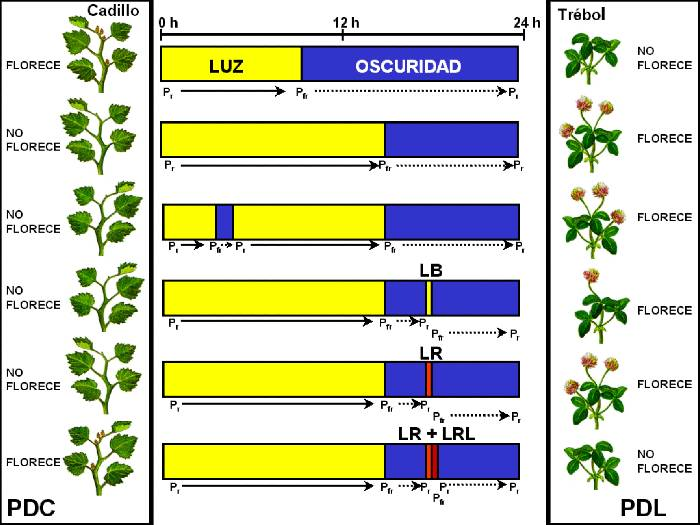
\includegraphics[width=0.5\textwidth]{fv10.jpg}
  \caption{Efecto que tiene la interrupción del período de oscuridad en plantas de día corto (cadillo) y de día largo (trébol).}
  \label{fv10}
\end{figure}

Como se ve en la primera barra, en condiciones de día corto (10 horas de luz y 14 de oscuridad) florece la PDC y no lo hace la  PDL. En  condiciones de día largo (14 de luz y 10 de oscuridad), segunda barra, florece la PDL pero no la PDC. En la tercera barra vemos como la interrupción del período luminoso con un corto período de oscuridad, en condiciones totales de día largo, no afectan para nada a la floración de las PDC (siguen sin florecer) y de las PDL (siguen floreciendo). En la cuarta barra observamos como una breve interrupción con luz blanca del período de oscuridad, cuando las condiciones son de día largo, tampoco influye en los resultados, y éstos son los esperados. 

En la quinta barra la interrupción del período de oscuridad con un pulso de luz roja, sigue sin alterar los resultados esperados. Sin embargo, en la barra sexta, vemos como la interrupción del período de oscuridad con pulsos alternos de luz roja y roja lejana, si afecta  a la floración siempre y cuando el último pulso sea de luz roja lejana, ya que esta convierte toda la forma $P_{fr}$ que aún permanece en la forma $P_r$ con lo que se impide la floración en la PDL.  
\begin{table}[h!]
    \centering
    \begin{tabular}{@{}ccc@{}}
    \toprule
    \multicolumn{3}{c}{Niveles óptimos de iluminación para cultivos} \\ \midrule
    Especie           & Int. Luz (lux)        & Duración             \\
    Tomate            & 10000-40000           & Día intermedio       \\
    Lechuga           & 12000-30000           & Día largo            \\
    Clavel            & 15000-45000           & Día intermedio       \\
    Rosa              & 100000                & Día intermedio       \\
    Crisantemo        & 75000-95000           & Día corto            \\ \bottomrule
    \end{tabular}
    \caption{Niveles óptimos de iluminación para cultivos}
    \label{tabfv6}
\end{table}

\begin{table}[h!]
    \centering
    \begin{tabular}{@{}cc@{}}
    \toprule
    Condiciones de iluminación & Porcentaje de germinación \\ \midrule
    Oscuridad                  & 20                        \\
    Luz blanca                 & 92                        \\
    Roja (R)                   & 98                        \\
    Roja lejana (RL)           & 1                         \\
    R-RL                       & 2                         \\
    R-RL-R                     & 98                        \\
    R-RL-R-RL                  & 1                         \\
    R-RL-R-RL-R                & 98                        \\
    R-RL-R-RL-R-RL             & 1                         \\ \bottomrule
    \end{tabular}
    \caption{Efecto de la iluminación sobre la germinación de semillas de lechuga (Lactuca sativa sv. Grand Rapids)}
    \label{tabfv7}
\end{table}













